\chapter{Diskussion}

In diesem Kapitel wird analytisch auf die vorangegangenen Resultate eingegangen und die Schwellenbestimmung der Rater und Software evaluiert. Im Zuge dessen werden die in Kapitel 1.3 aufgeführten Fragen chronologisch beantwortet:
%
\begin{tabbing}
	Ist die Bestimmung der Schwellen mit dem metabolicscan realisierbar?\\
	Welche Methode ist optimal?\\
	Kann die VT2 mit den neuen Methoden genauer bestimmt werden, als mit RQ~=~1?
\end{tabbing}
%
Anschließend werden Limitationen und eventuelle Defizite der Durchführung sowie potentielle Fehlerquellen behandelt und diesbezüglich einige Vorschläge für die Firma cardioscan präsentiert.\\[1em]

\section{Nutzbarkeit des metabolicscan zur Bestimmung der ventilatorischen Schwellen}

Da mit den vier Methoden für alle Testpersonen Ergebnisse erzielt wurden, kann geschlussfolgert werden, dass der metabolicscan in Verbindung mit der \acs{CCPS} und Fahrradergometern zur Bestimmung der ventilatorischen Schwellen genutzt werden kann. Während der Messungen wurden keine Störungen oder Fehler der verbauten Sensoren festgestellt. Die maximal gemessene Atemfrequenz bei den Testmessungen betrug \SI{52,5}{\per\minute} und liegt damit innerhalb der Grenzen des \acs{O2}-Sensors. Mit \SI{136,27}{\litre\per\minute} befindet sich auch die maximal gemessene \acs{VE} unterhalb des Maximums des Flowsensors. Der metabolicscan wurde vor dem Projekt mithilfe eines Lungensimulators bei Atemfrequenzen zwischen \SIlist{6;50}{\per\minute} und unterschiedlichen Gaskonzentrationen kalibriert, weswegen ausgeschlossen werden kann, dass die Sensoren fehlerhaft waren. Zudem wurde jeder bisher produzierte metabolicscan geprüft und mithilfe der Ergebnisse eine Ausgleichskurve für die Flowmessung entwickelt, wie in die Gerätekalibrierung zu Beginn einer Messung implementiert ist. Dennoch können Abweichungen in der Messtechnik nicht vollkommen ausgeschlossen werden. Zusätzlich wurden Anfälligkeiten für probanden-, -anwender- sowie umweltbedingte Fehler festgestellt, welche zum Ende des Kapitels aufgegriffen werden.

\section{Evaluierung der Methoden zur Schwellenbestimmung}

Die Plots wurden bezüglich ihrer Qualität zunächst subjektiv und unbeeinflusst von anderen Personen in die Kategorien Gut und Kritisch einsortiert. Plots, die optisch mithilfe einer jeweiligen Methode direkt auszuwerten waren und außerdem keine schwerwiegenden Artefakte aufwiesen, wurden als gut deklariert. In die Rubrik Kritisch kamen jene Graphen, die beispielsweise unregelmäßige Kurvenverläufe aufwiesen und dadurch nur sehr differenziert evaluiert werden konnten. Tab. \ref{tab:tabelle7} zeigt die Kategorien und Zuordnungen. Die jeweilige Menge an Graphen wurde in die zwei Spalten Gut und Kritisch eingeordnet. 
%
\begin{table}[H]
	\begin{center}
		\caption{Kategorisierung der Plots nach Qualität}
		\medskip
		\begin{tabulary}{\textwidth}{L L C C}
			\toprule
			& & Gut & Kritisch \\
			\midrule
			\midrule
			\multirow{3}{1.5cm}{\textbf{VT1}} & V-Slope & 7 & 21 \\
			& \acs{EQO2} & 13 & 15 \\
			\cmidrule{2-4}
			& \textsl{Summe} & 20 (36 \%) & 36 (64 \%) \\
			\midrule
			\multirow{3}{1.5cm}{\textbf{VT2}} & \acs{EQCO2} & 21 & 7 \\
			& \acs{VE}/\acs{VCO2} & 15 & 13 \\
			\cmidrule{2-4}
			& \textsl{Summe} & 36 (64 \%) & 20 (36 \%) \\
			\bottomrule
		\end{tabulary}
		\label{tab:tabelle7}
	\end{center}
\end{table}
%
Mit 64~\% wurde der Großteil aller Plots zur Bestimmung der VT1 als kritisch bewertet. 21 von 28 und damit 75~\% der V-Slope-Graphen war optisch kritisch. Mit 15 von 28 bzw. 54~\% wurde auch die absolute Mehrheit der \acs{EQO2}-Kurven so bewertet. Bei den Methoden zur VT2-Bestimmung fiel die Wertung andersherum aus und 75~\% der \acs{EQCO2}- und 54~\% der \acs{VE}/\acs{VCO2}-Plots wurden in die Kategorie Gut eingeordnet.

\subsection{Evaluierung der V-Slope-Methode}
%
\subsubsection{Gute Plots}

Es wurden die V-Slope-Plots als gut deklariert, die eine differenzierbare Steigung besaßen, sodass die Identifizierung eines Knickpunktes nicht durch zusätzliche Schwankungen erschwert wurde. Ein Beispiel dafür ist in Abb. \ref{pic:pic15} zu sehen. Dort konnte der \acs{VCO2}-Anstieg optisch eindeutig abgelesen werden und die Bestimmungen der Rater und Software differieren für die VT1 lediglich um maximal \SI{4}{\per\minute} (siehe Tab. \ref{tab:tabelle5}).

\subsubsection{Kritische Plots}

Wenn die V-Slopes und die zugeordneten \acs{HF}-Kurven nicht differenzierbar waren, wie beispielsweise ist den Plots in Abb. \ref{pic:pic18} und Abb. \ref{pic:pic19} erkennbar ist, war die subjektive Bestimmung der VT1 erschwert. Diese Problematik trat relativ häufig auf und wurde auch vom 2. Rater moniert. Es lagen jedoch auch Grafiken vor, bei denen die Plots zwar differenzierbar waren, aber dennoch mehrere Schwankungen aufwiesen.\\
Ein Beispiel hierfür ist die Grafik von Proband 8m. In Abb. \ref{pic:pic18} ist ein nicht differenzierbarer V-Slope zu sehen, der mehrere Knickpunkte enthält. Eine Vielzahl an solchen Punkten begünstigt eine große Varianz an Werten für die VT1. Während Rater 1 den ersten Anstieg in der 2. Stufe bei \SI{120}{\per\minute} beobachtete, wurde er laut Rater 2 erst nach den Schwankungen der Werte in Stufe 6 bei \SI{155}{\per\minute} erkennbar. Die kritische Bewertung des Plots wird dadurch belegt. Abb. \ref{subpic:pic1} zeigt hierzu, dass Rater 1 und Rater 2 häufiger, wie bei Proband 8m, zu unterschiedlichen Ergebnissen kamen.\\
Auch differenzierbare und stetig steigende V-Slopes, die jedoch viele Messpunkte besaßen und dadurch stärker geglättet wurden, brachten ungleiche Ergebnisse durch Rater und Software hervor. Für Proband 9m bestimmte Rater 1 die VT1 früher als Rater 2 und die Software. Bei Betrachtung von Abb. \ref{pic:pic19} fällt auf, dass die Kurvenverläufe allgemein recht eben sind. Hier wird ein Vorteil der algorithmischen Auswertung deutlich, da die Software die größte Steigungsänderung mathematisch und daher eindeutig bestimmt. Allerdings erkennt sie Software keine eventuellen Ausreißer und kann den Trainingszustand einer Person nicht bewerten, der die Rater dazu veranlassen konnte, die VT1 im späteren Messverlauf zu vermuten. 21 von 28 V-Slope-Grafiken waren aufgrund dieser Gründe kritisch, was durch das Diagramm in Abb. \ref{subpic:pic1} und die darin sichtbaren Abweichungen zwischen den Schwellenbestimmung belegt werden kann. Es ist im durch viele hellrote Schraffuren im Diagramm zu erkennen, dass der 2. Rater die VT1 meistens später bzw. bei höheren \acs{HF} bestimmte. Aus den gemittelten Werten für die VT1 der Rater und der algorithmischen Bestimmung wurde der Korrelationskoeffizient r für den V-Slope berechnet:
%
\begin{flalign*}
r_{V-Slope} = 0,526
\end{flalign*}
%

\subsection{Evaluierung der \acs{EQO2}-Methode}

\subsubsection{Gute Plots}

Eine gut auszuwertende \acs{EQO2}-Kurve steigt nach ihrem Tiefpunkt stetig an. Dadurch kann der Tiefpunkt eindeutig mit der VT1 assoziiert werden. Dies kann z.B. in Abb. \ref{pic:pic15} im Plot von Probandin 6w beobachtet werden, bei der Rater 1 und 2 die VT1 gemäß Tab. \ref{tab:tabelle5} vergleichbar bei \SIlist{106;109}{\per\minute} detektierten. Auch die Software kam mit \SI{106}{\per\minute} zum gleichen Ergebnis. 

\subsubsection{Kritische Plots}

Die \acs{EQO2}-Kurven waren dann kritisch, wenn der Tiefpunkt erst im späten Messverlauf auftauchte oder aber mehrere Tiefpunkte auf optisch relativ gleicher Höhe identifizierbar waren und beim ersten dieser Punkte kein alleiniger Anstieg des \acs{EQO2} stattfand, sondern auch das \acs{EQCO2} zunahm.\\
Auch hierfür kann die Grafik von Proband 8m als Beispiel verwendet werden. Der Tiefpunkt der \acs{EQO2}-Kurve liegt in Abb. \ref{pic:pic18} erst zwischen Stufe 6 und 7. Hier bestimmte Rater 2 dementsprechend auch die VT1. Da allerdings an diesem Punkt auch die \acs{EQCO2}-Kurve ansteigt und ein sehr leichter Anstieg der \acs{EQO2}-Kurve bereits nach Stufe 2 auftritt, wo das \acs{EQCO2} noch nicht zunimmt, wurde die VT1 von Rater 1 und auch von der Software dort identifiziert.\\
Ein weiteres Beispiel einer solchen Differenz zwischen den Ratern liegt bei Proband 21m vor (siehe Abb. \ref{subpic:pic2}). Erneut kann diese durch die Schwankungen des \acs{EQO2} in der entsprechenden Abb. \ref{pic:pic21} begründet werden. Rater 1 und Software nahmen hier auch den ersten \acs{EQO2}-Anstieg als die VT1 an, während Rater 2 die Schwelle am tatsächlichen Wertetiefpunkt der Kurve bestimmte.
%
\begin{flalign*}
 r_{EQO_2} = 0,464
\end{flalign*}
%
\subsection{Fazit zur VT1}

Letztlich zeigen die behandelten Beispielplots und die Diagramme in Abb. \ref{pic:pic23} und \ref{pic:pic24}, dass die Ergebnisse häufiger stark differieren und oftmals kein eindeutiger Bereich für die VT1 mittels V-Slope und \acs{EQO2} bestimmt werden kann. Die Ergebnisse beider Methoden weisen jeweils eine \acs{SD} von $\pm$14 \si{\per\minute} auf. Die gemittelte Differenz zwischen Ratern und Software fällt bei der \acs{EQO2}-Methode größer aus, was an zwei sehr großen Differenzen mit \SIlist{46,50}{\per\minute} liegt, die den Gesamtdurchschnitt bei 28 Probanden stark beeinflussen. Die beiden Korrelationskoeffizienten liegen relativ mittig von null und eins und belegen somit, dass die algorithmischen sowie durch Rater bestimmten VT1 der Testmessungen aufgrund der häufig starken Differenzen nur bedingt in Zusammenhang zu bringen sind und die verwendeten Methoden dementsprechend mit dieser Art der Durchführung einer Leistungsdiagnostik nicht als optimal bezeichnet werden können.

\subsection{Evaluierung der \acs{EQCO2}-Methode}

\subsubsection{Gute Ergebnisse}

Die Attribut "´gut"' beim \acs{EQCO2} galt, wenn im fortgeschrittenen Messverlauf nach ihrem Tiefpunkt ein deutlicher Anstieg der Kurve beobachtet werden konnte. Abb. \ref{subpic:pic3} zeigt, dass die Differenzen zwischen den beiden Ratern und auch zwischen den Ratern und der Software im Allgemeinen relativ gering waren. 

\subsection{Fazit zur VT2}

Bei den Werten für die VT2 differieren die Ergebnisse deutlich weniger, wie Abb. \ref{pic:pic25} andeutet. Am erfolgreichsten fiel die VT2-Bestimmung mittels \acs{EQCO2}-Anstieg aus, was mit  belegt werden kann. Lediglich bei fünf Probanden können Differenzen >\SI{10}{\per\minute} beobachtet werden (siehe Abb. \ref{pic:pic26}). Dabei bestimmte die Software die VT2 meistens ein wenig später als die Rater, was an hellgrünen Schraffuren in Abb. \ref{pic:pic25} zu erkennen ist. Erklären lässt sich dies z.B. anhand von Abb. \ref{pic:pic18} bei Proband 8m. Hier sind Schwankungen der \acs{EQCO2}-Steigung zu sehen, sodass die Kurve im letzten Drittel der Messung sogar zweimal ansteigt und zwischendurch einmal abfällt. So kam es zu unterschiedlichen Schwellen bei der manuellen Betrachtung durch die Rater.\\
Im Beispiel vom Probandin 6w in Abb. \ref{pic:pic17} ist sichtbar, dass die \acs{EQCO2}-Kurve stetig ansteigt. Rater 1 nahm die VT2 bereits beim ersten zeitlichen Anstieg nach Stufe 5 an. Software sowie Rater 2 wählten erst den überproportionalen Anstieg des \acs{EQCO2} nach Stufe 7 als die VT2. Die algorithmische Bestimmung erfolgt nach mehreren Schleifen, in denen Ausreißer bei der Steigung sowie die Referenzwerte der HUNT 3 Studie abgeglichen werden. Dieser Abgleich sorgt dafür, dass gelegentlich nicht der absolut erste \acs{EQCO2}-Anstieg markiert wird. Abb. \ref{pic:pic26} zeigt jedoch deutlich, dass große Differenzen zwischen den Instanzen recht selten sind und die Ergebnisse im Gesamtbild am meisten miteinander korrelieren.

\begin{figure}[H]
	\centering
	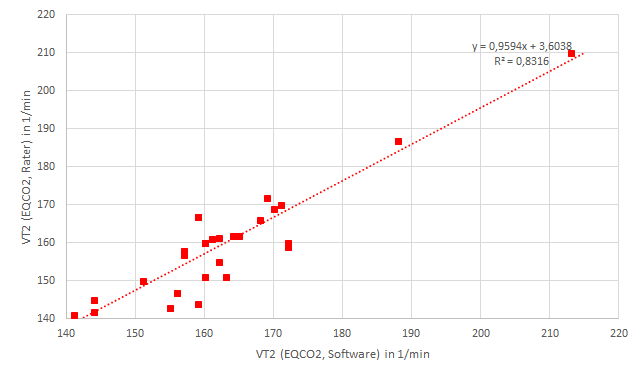
\includegraphics[scale=0.7]{Bilder/r_eqco2}
	\caption[Korrelation der \acs{EQCO2}-Ergebnisse von Ratern und Software]{Korrelation der Ergebnisse für die VT2 mit \acs{EQCO2} von Ratern und Software in Form einer Regressionsgeraden; aufgetragen wird die gemittelte VT2 gegenüber der VT2 der Software in \si{\per\minute}}
	\label{pic:pic28}
\end{figure}

Abb. \ref{pic:pic28} zeigt anhand einer Regressionsgeraden mit einem Bestimmtheitsmaß $R^2=0,83$, dass die subjektiven VT2 der Rater mit den referenzierten VT2 des Algorithmus in einen engen Zusammenhang gebracht werden können.
%
\begin{flalign*}
r_{EQCO_2} = 0,912
\end{flalign*}
%
Mit $0,912$ besitzt diese Methode im direkten Vergleich den größten Korrelationskoeffizienten.

\subsubsection{Kritische Ergebnisse}

Größere Unterschiede traten bei den Auswertungen mit \acs{VE}/\acs{VCO2} auf (siehe Abb. \ref{subpic:pic4}). Beispiele hierfür werden mit den Plots von 6w, 9m und 21m erörtert.\\
Bei Probandin 6w bestimmte Rater 1 die Schwelle im Vergleich zu Rater 2 und Software etwas früher. Abb. \ref{pic:pic17} zeigt, dass der Graph in Feld 4 von Beginn an weitestgehend linear ansteigt. Rater 1 beobachtete den ersten überproportionalen Anstieg der \acs{VE} in Stufe 5, Rater 2 und die Software erst in Stufe 7. Die Schwierigkeit bestand auch hier darin, den ersten Knickpunkt mit dem bloßen Auge zu identifizieren.\\
Abb. \ref{pic:pic19} von Proband 9m weist auch einen recht linearen Graphen in Feld 4 auf. Zudem liegen einige Messpunkte sehr dicht bei einander, was die subjektive Auswertung zusätzlich schwerer macht. Hier bestimmte der Algorithmus die VT2 eher als beide Rater.\\
Auch bei 21m unterscheiden sich die Ergebnisse von Rater 1 sowie Rater 2 und Software um eine Stufe. Abgesehen von den nicht differenzierbaren Messpunkten zwischen Stufe 3, 4 und 5, verläuft auch hier \acs{VE}/\acs{VCO2} in Feld 4 einigermaßen linear und der erste überproportionale Anstieg war der kritische Parameter.\\
Für die Auswertung von \acs{VE}/\acs{VCO2} lässt sich schlussfolgern, dass sie, ähnlich dem V-Slope, in Verbindung mit Mittelwerten und Stufentests erschwert wird, da der Graph anfällig für Artefakte ist. Eine \acs{SD} von $\pm$11 \si{\per\minute} zeigt, dass häufig keine eindeutigen Ergebnisse erzielt werden. Die Software birgt auch bei dieser Methode allerdings den Vorteil, dass die mathematische Bestimmung von Steigungsänderungen gut gelingt und die Methode somit für Vergleiche nutzbar wird. Die Ergebnisse liefern folgenden Korrelationskoeffizienten:
%
\begin{flalign*}
r_{\dot{V}E/\dot{V}CO_2} = 0,816
\end{flalign*}
%

\section{Problematik von RQ = 1}

Tab. \ref{tab:tabelle6} beweist sehr deutlich, dass die Methode RQ = 1 zur alleinigen Bestimmung der VT2 nicht valide ist. In Kapitel 1.3 wurde erwähnt, dass der RQ einst häufig zu früh den Wert eins überschritt und die Schwellenbestimmung dadurch fehlerhaft wurde. Dieser Fall trat bei den Ergebnissen der 28 Tests nicht auf. Dies ist jedoch dadurch begründet, dass durch cardioscans Entwicklung Ausgleichsgeraden in den Algorithmus implementiert wurden. Darüber hinaus wurde vor Start des Projektes ein Befehl aus der Ansteuerung der metabolicscan entfernt, der bewirkt hatte, dass dieser sich zwischen den einzelnen Belastungsstufen rekalibriert. Da jedoch bei einer Spiroergometrie durch den Probanden mehr \acs{CO2} exspiriert wird und die Räumlichkeiten währenddessen nicht belüftet werden, um Störungen des Flowsensors zu vermeiden, steigt entsprechend die \acs{CO2}-Konzentration der Luft. Dies konnte gemessen werden und wirkte sich somit auf die Kalibrierung des Geräts aus, sodass ungewollte Drifts in der RQ-Kurve entstanden.\\
Bei 9 von 28 Personen stieg der Wert stattdessen gar nicht über eins, sodass die VT2 gar nicht bestimmt werden konnte. Hier ließe sich diskutieren, ob diese Personen tatsächlich kardiorespiratorisch ausbelastet waren, oder den Test wegen muskulärer Erschöpfung beendet haben. Dennoch konnte bei diesen neun Probanden mit \acs{EQCO2} sowie \acs{VE}/\acs{VCO2} die VT2 bestimmt werden. Bei zehn Personen, bei denen mit der Referenzmethode eine VT2 definiert werden konnte, weichen die Werte jedoch von den übrigen Methoden mit \SI{10}{\per\minute} oder mehr ab. Darüber hinaus wurden für den MATLAB-Algorithmus bereits Ausgleichskurven für den RQ implementiert. Diese sorgen jedoch nicht dafür, dass die Mehrheit der Messergebnisse mit den übrigen Methoden vergleichbar wird. Der Algorithmus wird künftig aus der \acs{CCPS} entfernt und durch die genauere \acs{EQCO2}-Methode ersetzt.

\section{Plausibilitätsprüfung der Messwerte}

Für die Spiroergometrie existieren keine validen Methoden zur Plausibilitätskontrolle der Messwerte. Empfohlen wird stattdessen zur groben Abschätzung der Vergleich von \acs{VE}-, \acs{VO2}- und Belastungszunahme, da zwischen diesen Parametern bis zum Erreichen der VT1 eine gewisse physiologische Proportionalität besteht. Für diese Abschätzung sollen zwei Faustformeln in der klinischen Spiroergometrie nutzbar sein, wobei $n$ die Anzahl der gefahrenen Stufen sei~\cite{Ruehle.2012}:
%
\begin{flalign}
\dot{V}E_{max}\hspace{1mm} \text{in \si{\litre\per\minute}} &= \SI{9}{\litre\per\minute} + n * \SI{9}{\litre\per\minute} \pm 10 \%
\label{eq:formel14}\\[1em]
\dot{V}O_{2max}\hspace{1mm} \text{in \si{\milli\litre\per\minute}} &= 5 * \left\lbrace m\right\rbrace \text{in \kilogram} * W_{max}\hspace{1mm} \text{in \watt} * \SI{10}{\milli\litre\per\minute} \pm 10 \%
\label{eq:formel15}
\end{flalign}
%
\acs{VE} und \acs{VO2} sollen demnach einen idealerweise linearen Verlauf über die Leistung annehmen. Da die Berechnungen jedoch kaum anthropometrischen Daten oder individuellen Trainingszustände einbeziehen, wurde auf die mathematische Art der Überprüfung wegen der großen Varianz an Trainingszuständen in dieser Arbeit verzichtet. Allerdings kann mithilfe eines grafischen Vergleichs der Parameter der Verlauf einer Messung analysiert und bewertet werden.\\
Abb. \ref{pic:pic15} in Kapitel 3.1.1 zeigt in Feld 5 und 6 einen solchen Messverlauf für die \acs{VE} und \acs{VO2} im Falle der Probandin 6w. In Ruhe beträgt die \acs{VE} ca. \SI{9}{\litre\per\minute}, steigt danach tatsächlich um ca. \SI{9}{\litre\per\minute}, doch danach flacht die Steigung ein wenig ab. Dennoch steigen die Graphen stetig an, weswegen von einem guten Messverlauf ausgegangen wird. Nicht bei allen Probanden jedoch hatten die Plots eine solche Form.\\
In Abb. \ref{pic:pic21} sind Plots mit Artefakten zu sehen. Zwischen den Stufen 2 und 6 schwanken die Messwerte sowohl für die \acs{VE}, als auch für die \acs{VO2} sehr stark. Es sind mehrere Abfälle des Graphen an Stelle eines stetigen Anstiegs sichtbar. Da die \acs{VO2} mathematisch von der \acs{VE} abhängt (vgl. Kapitel 1.2.1), ist von einem Messfehler der \acs{VE} auszugehen. Diese ist abhängig vom Atemzugvolumen sowie der \acs{AF}. Da auch diese beiden Parameter physiologisch bedingt ansteigen, ist es sehr wahrscheinlich, dass während der Messungen zwischen den betroffenen Stufen weniger Atemzüge korrekt erfasst wurden. Dies kann beispielsweise daran liegen, dass Probleme mit dem Mundstück bestanden. 7 der 28 Probanden empfanden die Ergonomie des Mundstücks als unangenehm und deuteten nach dem Test an, dass dieses die Atmung gerade zu Beginn einer Messphase erschwert habe.\\
Auch Proband 21m hatte Schwierigkeiten mit dem Mundstück und konnte dieses in mehreren Stufen nicht rechtzeitig für eine korrekte Atemzugerfassung platzieren. Einer weiteren Probandin rutschte das Mundstück bei erhöhter Belastung während einer Messung mehrmals aus dem Mund. Somit konnten die Graphen Aufschluss über den Erfolg einer Messphase zwischen zwei Stufen geben und bei der Analyse der restlichen Graphen zur Schwellenbestimmung unterstützen. Zum Beispiel konnten die Messpunkte der Atemäquivalente im 2. Feld der 6-Felder-Grafik direkt mit dem \acs{VE}/Watt-Plot verglichen und so verifiziert werden.\\
In Abb. \ref{pic:pic21} ist beispielsweise zu sehen, dass auch in den vier Feldern zur Schwellenbestimmung die Kurven zwischen positivem und negativem Verlauf schwanken. Im V-Slope in Feld 1 sinken die \acs{VO2} und \acs{VCO2} zwischen Messpunkt 3 und 4 sowie 4 und 5 wieder ab. Dies trifft auch auf die \acs{VE} und \acs{VCO2} in Feld 4 zu. Analog dazu sinkt die \acs{VE} im 5. Feld. Derartige Artefakte können mit der Mundstück-Problematik belegt werden, da die Messzeit mit \SI{30}{\second} gleichbleibend war. Durch den Verlust des Mundstücks innerhalb einer Messung wird auch die Anzahl der registrierten Atemzüge reduziert, sodass die Berechnung der \acs{AF} und \acs{VE} durch die Software fehlerhaft und der Durchschnitt im Gesamtverlauf stark beeinflusst wird.\\
In Feld 2 von Abb. \ref{pic:pic21} fällt bei Betrachtung der blauen \acs{EQO2}-Kurve auf, dass der Tiefpunkt sehr spät nach der 5. Stufe auftrat. Vergleicht man die Kurven mit Feld 5 und 6, kann auch dies durch Messfehler begründet werden, da auch in der 5. Stufe wieder ein Abfall der \acs{VE} beobachtet werden kann. Diese Plots wurden schließlich bei der Evaluierung der Ergebnisse berücksichtigt, um Unterschiede zwischen den Ratern und der Software zu erörtern und nachträglich diskutieren zu können, welche charakteristischen Punkte in den Plots tatsächlich durch die pathophysiologischen Veränderungen der Respiration und Ventilation bedingt waren.

\section{Potentielle Fehlerquellen bei der Spiroergometrie}

\subsection{Probandenbedingte Faktoren}

Bei der Spiroergometrie können Probanden die Ergebnisse negativ beeinflussen, indem sie ihre Atmung durch die ungewohnten Bedingungen stark verändern, sodass diese unphysiologisch wird. Bei wenigen Personen konnte beobachtet werden, dass sie zu Beginn der Leistungsdiagnostik eine recht hohe \acs{VE} besaßen und die \acs{AF} schnell zunahm. Dies lag vor allem am Mundstück und dem Bakterienfilter. Durch diesen erhöht sich der Atemwiderstand, dessen Höhe von jeder Person subjektiv anders wahrgenommen wird. Dadurch neigten die Probanden dazu, tiefer und gleichzeitig schneller zu atmen. Infolgedessen stieg die \acs{VE} relativ zur \acs{VO2} höher, da der Körper zu diesem Zeitpunkt noch nicht die große Menge an aufgenommenem \acs{O2} verwerten konnte. Des Weiteren können Fehler entstehen, wenn Personen das Mundstück nicht rechtzeitig zu Munde führen. Die Dauer der Messphase beträgt stets \SI{30}{\second}. Zu Beginn einer Leistungsdiagnostik bei geringer Leistung ist die \acs{AF} bei den meisten gesunden Menschen noch recht niedrig. Die durchschnittliche \acs{AF} eines Erwachsenen in Ruhe beträgt ca. \SIrange{7}{20}{\per\minute}~\cite{Larsen.2017}. Kommt es zu Problemen mit dem Mundstück, sodass gewisse Schwellwerte bei der Atemzugerkennung der Software nicht überschritten und weniger Atemzüge erfasst werden, wird die gemittelte \acs{AF} und dadurch auch die \acs{VE} kleiner. Das wiederum kann zu veränderten Plots führen, wenn auf einen kleineren Mittelwert in der nächsten Stufe ein normaler folgt, wodurch die Steigung zwischen diesen zwei Punkten verfälscht wird und nicht mehr den ventilatorischen Reaktionen des Körpers entspricht. Zuletzt muss die Ernährung unmittelbar vor einer Spiroergometrie berücksichtigt werden (siehe Kapitel 2.1.2). Zwar wird zukünftig der RQ nicht mehr für die Schwellenbestimmung verwendet, jedoch sollte der Grund-Laktat-Gehalt nicht durch erhöhte Zuckerzufuhr erhöht werden, um die Ausgangsbedingungen in Bezug auf die \acs{VCO2} zu normalisieren.

\subsection{Anwenderbedingte Faktoren}

Durch den Anwender der Spiroergometrie können ebenfalls Fehler verursacht werden. Beispielsweise kann oben genannter zeitlicher Verzug auch entstehen, wenn der Anwender dem Probanden das Mundstück zu spät reicht, sodass die Atemzugerfassung ebenfalls verfälscht wird. Schon eine falsche Vorbereitung der Belastungsphase kann zu Fehlern führen, wenn z.B. die Sattelhöhe nicht korrekt justiert oder ein unpassendes Belastungsprotokoll bestimmt wurde. Es ist wichtig, dass der Anwender im Vorwege den Trainingszustand einer Person korrekt einschätzen kann, um entsprechende Anpassungen am Protokoll vorzunehmen. Allerdings ist hier auch die deutliche Kommunikation mit dem Probanden zwingend erforderlich.

\subsection{Umweltbedingte Faktoren}

Wie in Kapitel 2.1.2 erwähnt, sind die Messbedingungen für eine Respirationsanalyse einzuhalten. Raumtemperatur und \acs{CO2}-Gehalt in der Luft wirken sich auf die \acs{HF} und \acs{La-}-Kinetik aus, was ebenfalls im Falle einer Nichtbeachtung zu Fehlern führt. Jedoch wurde der Raum vor jedem Test belüftet und die Temperatur im Toleranzbereich zwischen \SIrange{18}{22}{\degreeCelsius} gehalten. Die \acs{CO2}-Belastung der Atemluft in $10^{-6}$ (parts per million) wurde durch ein Messgerät sehr genau überprüft, um sicherzustellen, dass die Kalibrierung des metabolicscan vor jedem Test auf denselben Grundbedingungen basierte.

\section{Limitation}

Das Pilotprojekt war limitiert durch eine relativ kleine Teilnehmerzahl und dadurch sehr ungleiche Verteilung der unterschiedlichen Probandengruppen. Um die Aussagekraft der Ergebnisse zu erhöhen und diese beispielsweise besser mit der HUNT 3 Studie vergleichen zu können, wäre eine deutlich größere Probandengruppe notwendig gewesen. Die Evaluierung war auch durch eine kleine Menge an wertenden Personen und einen gleichzeitigen Mangel an validen Referenzwerten eingeschränkt. Generell sind Normwerte im Bereich der Sportwissenschaft schwer zu definieren, da die Individualität an Zuständen zu groß ist. Dies bedeutet, dass bei der Analyse der individuellen Leistungsfähigkeit noch sensibler auf eventuelle Einflussfaktoren eingegangen werden muss, als beispielsweise bei einer rein medizinischen Lungenfunktionsmessung, der einige Normbereiche für z.B. das \ac{FEV1} oder \ac{FVC} zu Grunde liegen, welche anatomisch abgegrenzt sind.

\section{Fazit und Handlungsempfehlung}

Ausgehend von den Ergebnissen dieser Arbeit wurde mit dem \acs{EQCO2} eine neue Methode für die VT2-Bestimmung erarbeitet, welche zukünftig als Algorithmus die Basis für die Auswertung durch die \acs{CCPS} darbieten kann. In Verbindung mit dem Trainingszonenmodell nach Wilfried Kindermann können mit dieser Methode die Ziele der Firma cardioscan umgesetzt werden. Das Leistungsdiagnostik-Setup bietet jedoch Optimierungsmöglichkeiten. Zum Ersten wären eventuell Alternativen zu dem Mundstück, z.B. in Form einer Maske sinnvoll, da die Ergonomie des Mundstücks moniert wurde. Hier könnten weitere Tests mit alternativen Komponenten durchgeführt werden. Zum Zweiten gestaltet sich die Mittelung der Messwerte über die Gesamtanzahl an Atemzügen pro Stufe als nicht optimal, da dadurch die vorangegangen beschriebenen Verfälschung der Plots auftreten können. Eine gänzliche "`breath-by-breath"'-Auswertung jedes Atemzugs sollte wegen der zu großen Datenmenge zwar auch nicht in Betracht bezogen werden, jedoch könnten alternative Mittelungsverfahren (z.B. die "`gleitende"' Mittelung~\cite{Kroidl.2015}) getestet werden.\\
Die algorithmische Auswertung könnte für die anschließende Interpretation optimiert werden, indem z.B. ein Algorithmus programmiert wird, der ein Abflachen der \acs{HF}-Kurve zum Ende einer Leistungsdiagnostik überprüft. Dies könnte den Anwender dabei unterstützen, zu bewerten, ob eine Person tatsächlich ausbelastet war. In der HUNT 3 Studie wurde ermittelt, bei wie viel Prozent der \acs{HFmax} die VT2 einer Person erreicht worden war. Eine abflachende \acs{HF}-Kurve wäre ein Indikator für das Erreichen der \acs{HFmax}. Durch einen Vergleich der \acs{HF} bei der VT2 und der \acs{HFmax} könnten Ergebnisse zusätzlich evaluiert werden.\\
Zum Abschluss bleibt zu erwähnen, dass, trotz algorithmischer Auswertung einer Spiroergometrie, eine Interpretation der Ergebnisse seitens einer Person mit Fachwissen unabdingbar ist. Die gezeigten Grafiken, anhand derer die Schwellen bestimmt wurden, bieten lediglich die Grundlage und müssen in ein optimiertes Interface der \acs{CCPS} implementiert werden. Die komplette Thematik der Atemgasanalyse ist im Allgemeinen sehr komplex und sollte daher nicht von ungeschultem Personal behandelt werden. cardioscan betreibt für alle diagnostischen Anwendungen eine Academy, welche in regelmäßigen Intervallen Seminare und Workshops durch Schulungsreferenten und -referentinnen beim Kunden durchführen lässt. Bei diesen Seminaren sollten auch die Feinheiten der Vorbereitung behandelt werden. Die Software könnte die Anwender auch auf diesem Wege unterstützen, indem z.B. der Timer im Interface durch einen Hinweis ergänzt wird, der daran erinnert, das Mundstück zur Messung vorzubereiten, um Messfehler zu reduzieren.


\nocite{*}

%\printnomenclature

%\bibliography{Referenzen}
\printbibliography